\documentclass[english,hidelinks, 11 pt, class=report,crop=false]{standalone}
\usepackage[T1]{fontenc}
%\usepackage[utf8]{inputenc}
\usepackage{lmodern} % load a font with all the characters
\usepackage{geometry}
\geometry{verbose,paperwidth=16.1 cm, paperheight=24 cm, inner=2.3cm, outer=1.8 cm, bmargin=2cm, tmargin=1.8cm}
\setlength{\parindent}{0bp}
\usepackage{import}
\usepackage[subpreambles=false]{standalone}
\usepackage{amsmath}
\usepackage{amssymb}
\usepackage{esint}
\usepackage{babel}
\usepackage{tabu}
\makeatother
\makeatletter

\usepackage{titlesec}
\usepackage{ragged2e}
\RaggedRight
\raggedbottom
\frenchspacing

\usepackage{graphicx}
\usepackage{float}
\usepackage{subfig}
\usepackage{placeins}
\usepackage{cancel}
\usepackage{framed}
\usepackage{wrapfig}
\usepackage[subfigure]{tocloft}
\usepackage[font=footnotesize,labelfont=sl]{caption} % Figure caption
\usepackage{bm}
\usepackage[dvipsnames, table]{xcolor}
\definecolor{shadecolor}{rgb}{0.105469, 0.613281, 1}
\colorlet{shadecolor}{Emerald!15} 
\usepackage{icomma}
\makeatother
\usepackage[many]{tcolorbox}
\usepackage{multicol}
\usepackage{stackengine}

\usepackage{esvect} %For vectors with capital letters

% For tabular
\usepackage{array}
\usepackage{multirow}
\usepackage{longtable} %breakable table

% Ligningsreferanser
\usepackage{mathtools} % for mathclap
%\mathtoolsset{showonlyrefs}

% sections without numbering in toc
\newcommand\tsec[1]{\phantomsection \addcontentsline{toc}{section}{#1}
	\section*{#1}}

% index
\usepackage{imakeidx}
\makeindex[title=Indeks]

%Footnote:
\usepackage[bottom, hang, flushmargin]{footmisc}
\usepackage{perpage} 
\MakePerPage{footnote}
\addtolength{\footnotesep}{2mm}
\renewcommand{\thefootnote}{\arabic{footnote}}
\renewcommand\footnoterule{\rule{\linewidth}{0.4pt}}
\renewcommand{\thempfootnote}{\arabic{mpfootnote}}

%colors
\definecolor{c1}{cmyk}{0,0.5,1,0}
\definecolor{c2}{cmyk}{1,0.25,1,0}
\definecolor{n3}{cmyk}{1,0.,1,0}
\definecolor{neg}{cmyk}{1,0.,0.,0}


\newcommand{\nreq}[1]{
\begin{equation}
	#1
\end{equation}
}


% Equation comments
\newcommand{\cm}[1]{\llap{\color{blue} #1}}


\usepackage[inline]{enumitem}
\newcounter{rg}
\numberwithin{rg}{chapter}


\newcommand{\reg}[2][]{\begin{tcolorbox}[boxrule=0.3 mm,arc=0mm,colback=blue!3] {\refstepcounter{rg}\phantomsection \large \textbf{\therg \;#1} \vspace{5 pt}}\newline #2  \end{tcolorbox}\vspace{-5pt}}
\newcommand{\regdef}[2][]{\begin{tcolorbox}[boxrule=0.3 mm,arc=0mm,colback=blue!3] {\refstepcounter{rg}\phantomsection \large \textbf{\therg \;#1} \vspace{5 pt}}\newline #2  \end{tcolorbox}\vspace{-5pt}}
\newcommand{\words}[1]{\begin{tcolorbox}[boxrule=0.3 mm,arc=0mm,colback=teal!3] #1  \end{tcolorbox}\vspace{-5pt}}

\newcommand\alg[1]{\begin{align*} #1 \end{align*}}

\newcommand\eks[2][]{\begin{tcolorbox}[boxrule=0.3 mm,arc=0mm,enhanced jigsaw,breakable,colback=green!3] {\large \textbf{\ekstitle #1} \vspace{5 pt}\\} #2 \end{tcolorbox}\vspace{-5pt} }

\newcommand{\st}[1]{\begin{tcolorbox}[boxrule=0.0 mm,arc=0mm,enhanced jigsaw,breakable,colback=yellow!12]{ #1} \end{tcolorbox}}

\newcommand{\spr}[1]{\begin{tcolorbox}[boxrule=0.3 mm,arc=0mm,enhanced jigsaw,breakable,colback=yellow!7] {\large \textbf{\sprtitle} \vspace{5 pt}\\} #1 \end{tcolorbox}\vspace{-5pt} }

\newcommand{\sym}[1]{\colorbox{blue!15}{#1}}

\newcommand{\info}[2]{\begin{tcolorbox}[boxrule=0.3 mm,arc=0mm,enhanced jigsaw,breakable,colback=cyan!6] {\large \textbf{#1} \vspace{5 pt}\\} #2 \end{tcolorbox}\vspace{-5pt} }

\newcommand\algv[1]{\vspace{-11 pt}\begin{align*} #1 \end{align*}}

\newcommand{\regv}{\vspace{5pt}}
\newcommand{\mer}{\textsl{\note}: }
\newcommand{\mers}[1]{{\footnotesize \mer #1}}
\newcommand\vsk{\vspace{11pt}}
\newcommand{\tbs}{\vspace{5pt}}
\newcommand\vs{\vspace{-11pt}}
\newcommand\vsb{\vspace{-16pt}}
\newcommand\br{\\[5 pt]}
\newcommand{\figp}[1]{../fig/#1}
\newcommand\algvv[1]{\vs\vs\begin{align*} #1 \end{align*}}
\newcommand{\y}[1]{$ {#1} $}
\newcommand{\os}{\\[5 pt]}
\newcommand{\prbxl}[2]{
\parbox[l][][l]{#1\linewidth}{#2
	}}
\newcommand{\prbxr}[2]{\parbox[r][][l]{#1\linewidth}{
		\setlength{\abovedisplayskip}{5pt}
		\setlength{\belowdisplayskip}{5pt}	
		\setlength{\abovedisplayshortskip}{0pt}
		\setlength{\belowdisplayshortskip}{0pt} 
		\begin{shaded}
			\footnotesize	#2 \end{shaded}}}
\newcommand{\fgbxr}[2]{
	\parbox[r][][l]{#1\linewidth}{#2
}}		

\renewcommand{\cfttoctitlefont}{\Large\bfseries}
\setlength{\cftaftertoctitleskip}{0 pt}
\setlength{\cftbeforetoctitleskip}{0 pt}

\newcommand{\bs}{\\[3pt]}
\newcommand{\vn}{\\[6pt]}
\newcommand{\fig}[1]{\begin{figure}[H]
		\centering
		\includegraphics[]{\figp{#1}}
\end{figure}}

\newcommand{\figc}[2]{\begin{figure}
		\centering
		\includegraphics[]{\figp{#1}}
		\caption{#2}
\end{figure}}
\newcommand{\arc}[1]{{
		\setbox9=\hbox{#1}%
		\ooalign{\resizebox{\wd9}{\height}{\texttoptiebar{\phantom{A}}}\cr\textit{#1}}}}

\newcommand{\sectionbreak}{\clearpage} % New page on each section

\newcommand{\nn}[1]{
\begin{equation*}
	#1
\end{equation*}
}

\newcommand{\enh}[1]{\,\textrm{#1}}

%asin, atan, acos
\DeclareMathOperator{\atan}{atan}
\DeclareMathOperator{\acos}{acos}
\DeclareMathOperator{\asin}{asin}

% Comments % old cm, ggb cm is new
%\newcommand{\cm}[1]{\llap{\color{blue} #1}}

%%%

\newcommand\fork[2]{\begin{tcolorbox}[boxrule=0.3 mm,arc=0mm,enhanced jigsaw,breakable,colback=yellow!7] {\large \textbf{#1 (\expl)} \vspace{5 pt}\\} #2 \end{tcolorbox}\vspace{-5pt} }
 
%colors
\newcommand{\colr}[1]{{\color{red} #1}}
\newcommand{\colb}[1]{{\color{blue} #1}}
\newcommand{\colo}[1]{{\color{orange} #1}}
\newcommand{\colc}[1]{{\color{cyan} #1}}
\definecolor{projectgreen}{cmyk}{100,0,100,0}
\newcommand{\colg}[1]{{\color{projectgreen} #1}}

% Methods
\newcommand{\metode}[2]{
	\textsl{#1} \\[-8pt]
	\rule{#2}{0.75pt}
}

%Opg
\newcommand{\abc}[1]{
	\begin{enumerate}[label=\alph*),leftmargin=18pt]
		#1
	\end{enumerate}
}
\newcommand{\abcs}[2]{
	\begin{enumerate}[label=\alph*),start=#1,leftmargin=18pt]
		#2
	\end{enumerate}
}
\newcommand{\abcn}[1]{
	\begin{enumerate}[label=\arabic*),leftmargin=18pt]
		#1
	\end{enumerate}
}
\newcommand{\abch}[1]{
	\hspace{-2pt}	\begin{enumerate*}[label=\alph*), itemjoin=\hspace{1cm}]
		#1
	\end{enumerate*}
}
\newcommand{\abchs}[2]{
	\hspace{-2pt}	\begin{enumerate*}[label=\alph*), itemjoin=\hspace{1cm}, start=#1]
		#2
	\end{enumerate*}
}

% Exercises


\newcounter{opg}
\numberwithin{opg}{section}

\newcounter{grub}
\numberwithin{opg}{section}
\newcommand{\op}[1]{\vspace{15pt} \refstepcounter{opg}\large \textbf{\color{blue}\theopg} \vspace{2 pt} \label{#1} \\}
\newcommand{\eksop}[2]{\vspace{15pt} \refstepcounter{opg}\large \textbf{\color{blue}\theopg} (#1) \vspace{2 pt} \label{#2} \\}

\newcommand{\nes}{\stepcounter{section}
	\setcounter{opg}{0}}
\newcommand{\opr}[1]{\vspace{3pt}\textbf{\ref{#1}}}
\newcommand{\oeks}[1]{\begin{tcolorbox}[boxrule=0.3 mm,arc=0mm,colback=white]
		\textit{\ekstitle: } #1	  
\end{tcolorbox}}
\newcommand\opgeks[2][]{\begin{tcolorbox}[boxrule=0.1 mm,arc=0mm,enhanced jigsaw,breakable,colback=white] {\footnotesize \textbf{\ekstitle #1} \\} \footnotesize #2 \end{tcolorbox}\vspace{-5pt} }


% tag exercises
\newcommand{\tagop}[1]{ 
{\small \color{Gray} #1} \os
}

% License
\newcommand{\lic}{
This book is part of the \net{https://sindrsh.github.io/openmathbooks/}{OpenMathBooks} project. OpenMathBooks © 2022 by Sindre Sogge Heggen is licensed under CC BY-NC-SA 4.0. To view a copy of this license, visit \net{http://creativecommons.org/licenses/by-nc-sa/4.0/}{http://creativecommons.org/licenses/by-nc-sa/4.0/}}

%referances
\newcommand{\net}[2]{{\color{blue}\href{#1}{#2}}}
\newcommand{\hrs}[2]{\hyperref[#1]{\color{blue}#2 \ref*{#1}}}
\newcommand{\refunnbr}[2]{\hyperref[#1]{\color{blue}#2}}


\newcommand{\openmath}{\net{https://sindrsh.github.io/openmathbooks/}{OpenMathBooks}}
\newcommand{\am}{\net{https://sindrsh.github.io/FirstPrinciplesOfMath/}{AM1}}
\newcommand{\mb}{\net{https://sindrsh.github.io/FirstPrinciplesOfMath/}{MB}}
\newcommand{\tmen}{\net{https://sindrsh.github.io/FirstPrinciplesOfMath/}{TM1}}
\newcommand{\tmto}{\net{https://sindrsh.github.io/FirstPrinciplesOfMath/}{TM2}}
\newcommand{\amto}{\net{https://sindrsh.github.io/FirstPrinciplesOfMath/}{AM2}}
\newcommand{\eksbm}{
\footnotesize
Dette er opppgaver som har blitt gitt ved sentralt utformet eksamen i Norge. Oppgavene er laget av Utdanningsdirektoratet. Forkortelser i parantes viser til følgende:
\begin{center}
	\begin{tabular}{c|c}
		E & Eksempeloppgave \\
		V/H & Eksamen fra vårsemesteret/høstsemesteret\\
		G/1P/1T/R1/R2 & Fag  \\
		XX & År 20XX \\
		D1/D2 & Del 1/Del 2
	\end{tabular}
\end{center}
Tekst og innhold kan her være noe endret i forhold til originalen.
}

%Excel og GGB:

\newcommand{\g}[1]{\begin{center} {\tt #1} \end{center}}
\newcommand{\gv}[1]{\begin{center} \vspace{-11 pt} {\tt #1}  \end{center}}
\newcommand{\cmds}[2]{{\tt #1}\\
	#2}

% outline word
\newcommand{\outl}[1]{{\boldmath \color{teal}\textbf{#1}}}
%line to seperate examples
\newcommand{\linje}{\rule{\linewidth}{1pt} }


%Vedlegg
\newcounter{vedl}
\newcounter{vedleq}
\renewcommand\thevedl{\Alph{vedl}}	
\newcommand{\nreqvd}{\refstepcounter{vedleq}\tag{\thevedl \thevedleq}}

%%% Writing code

\usepackage{listings}


\definecolor{codegreen}{rgb}{0,0.6,0}
\definecolor{codegray}{rgb}{0.5,0.5,0.5}
\definecolor{codepurple}{rgb}{0.58,0,0.82}
\definecolor{backcolour}{rgb}{0.95,0.95,0.92}

\newcommand{\pymet}[1]{{\ttfamily\color{magenta} #1}}
\newcommand{\pytype}[1]{{\ttfamily\color{codepurple} #1}}

\lstdefinestyle{mystyle}{
	backgroundcolor=\color{backcolour},   
	commentstyle=\color{codegreen},
	keywordstyle=\color{magenta},
	numberstyle=\tiny\color{codegray},
	stringstyle=\color{codepurple},
	basicstyle=\ttfamily\footnotesize,
	breakatwhitespace=false,         
	breaklines=true,                 
	captionpos=b,                    
	keepspaces=true,                 
	numbers=left,                    
	numbersep=5pt,                  
	showspaces=false,                
	showstringspaces=false,
	showtabs=false,                  
	tabsize=2,
	inputencoding=utf8,
	extendedchars=true,
	literate= {
		{å}{{\aa}}1 
		{æ}{{\ae}}1 
		{ø}{{\o}}1
	}
}

\lstset{style=mystyle}

\newcommand{\python}[1]{
\begin{tcolorbox}[boxrule=0.3 mm,arc=0mm,colback=white]
\lstinputlisting[language=Python]{#1}
\end{tcolorbox}}
\newcommand{\pythonut}[2]{
\begin{tcolorbox}[boxrule=0.3 mm,arc=0mm,colback=white]
\small 
%\textbf{Kode}
\lstinputlisting[language=Python]{#1}	
\vspace{11pt}
\textbf{Utdata} \\ \ttfamily
#2
\end{tcolorbox}}
%%%

%page number
%\usepackage{fancyhdr}
%\pagestyle{fancy}
%\fancyhf{}
%\renewcommand{\headrule}{}
%\fancyhead[RO, LE]{\thepage}

\usepackage{datetime2}
%%\usepackage{sansmathfonts} for dyslexia-friendly math
\usepackage[]{hyperref}




\begin{document}
{\Large Eksamen R1 Høsten 2023\hfill {\footnotesize Løsning fra \color{blue} \href{https://sindreheggen.wordpress.com/}{OpenMathBooks prosjektet}}}
\subsection*{Oppgave 1}	
Av produktregelen ved derivasjon har vi at
\alg{
f'(x) &= (x^2)'\ln x + x^2 (\ln x)'\\
&= 2x\ln x + x^2\frac{1}{x} \\
&= x(2\ln x+ 1)
}
\subsection*{Oppgave 2}
Vi har at
\alg{
&2\ln e = 2 \vn
&3\log 70=3\log 7 + 3\log 10 = 3\log 7+3>2  \vn
&e^{3\ln 2} = \left(e^{\ln 2}\right)^3=2^3=8
}
Da $\log 7<1 $, er $ 3\log 7+3<8 $, og dermed er
\[ 2\ln e<3\log 70<e^3\ln 2 \]
\subsection*{Oppgave 3}
\abc{
\item Vi har at
\alg{
	\vv{AB}&=[2-(-3), -2-(-1)]=[5, -1]\vn 
	\vv{BC}&=[3, 4]\vn
	\vv{AC}&=[8, 3]
}
Videre er
\alg{
	|\vv{AB}|&=\sqrt{5+(-1)^2}=\sqrt{26}\vn
	|\vv{BC}|&=\sqrt{25}\vn
	|\vv{AC}|&=\sqrt{73}
}
Dermed er $ BC $ kortest.
\item For to vektorer $ \vec{a} $ og $ \vec{b} $ har vi at $ \vec{a}\cdot\vec{b}\iff \angle(\vec{a}, \vec{b})=90^\circ$. Videre har vi at
\alg{
\vv{AB}\cdot\vv{BC}&=5\cdot3+(-1)4=11\vn
\vv{BC}\cdot\vv{AC}&= 36 \vn
\vv{AB}\cdot\vv{AC}&=37
}
Dermed er ingen av vinklene i trekanten $ 90^\circ $.
}

\subsection*{Oppgave 4}
\abc{
\item I skriptet: \\
Linje 1-2: Definerer $ f(x) $.\\
Linje 4-5: Definerer $ f'(x) $\\
Linje 6-7: Setter verdiene til $ h $ og $ a $\\
Linje 10-11: Kjører en while-loop som stopper når $ df(a,h)\geq 0 $, og som øker $ a $ med 1 for hver iterasjon. \vsk

Egil antar at $ f'(a)<0 $ for $ {a=0} $, og forsøker etterpå å finne $ a $-verdien hvor $ f(x) $ skifter fortegn. Hvis $ f'(x) $ skifter fra negativt til positivt fortegn i $ a $, vil dette være bunnpunktet til $ f $.

\item Å øke $ a $ med 1 gjør at Egil bare sjekker for $ a\in\mathbb{N} $. Han bør derfor øke $ a $ med en mye mindre verdi. Forslag for Linje 11:\\
\texttt{a = a + 0.01}
}
\newpage
\subsection*{Oppgave 1}
\abc{ 
\item Da potensfunksjoner ikke kan gå gjennom punktet $ (0, 0) $, bruker vi tallene i tabellen hvor konsentrasjonen er fratrekt 2,5. Ved regresjon får vi potensfunksjonene $ g(x) $. Da denne tilnærmet går gjennom alle punktene vi har lagt inn, ser $ g(x) $ ut til å være en god modell. $ f(t) $ fra oppgaven gjennkjenner vi som $ g(t)+2,5 $, og dermed er $ f $ en god modell for konsentrasjonen av stoffet.
\begin{figure}
	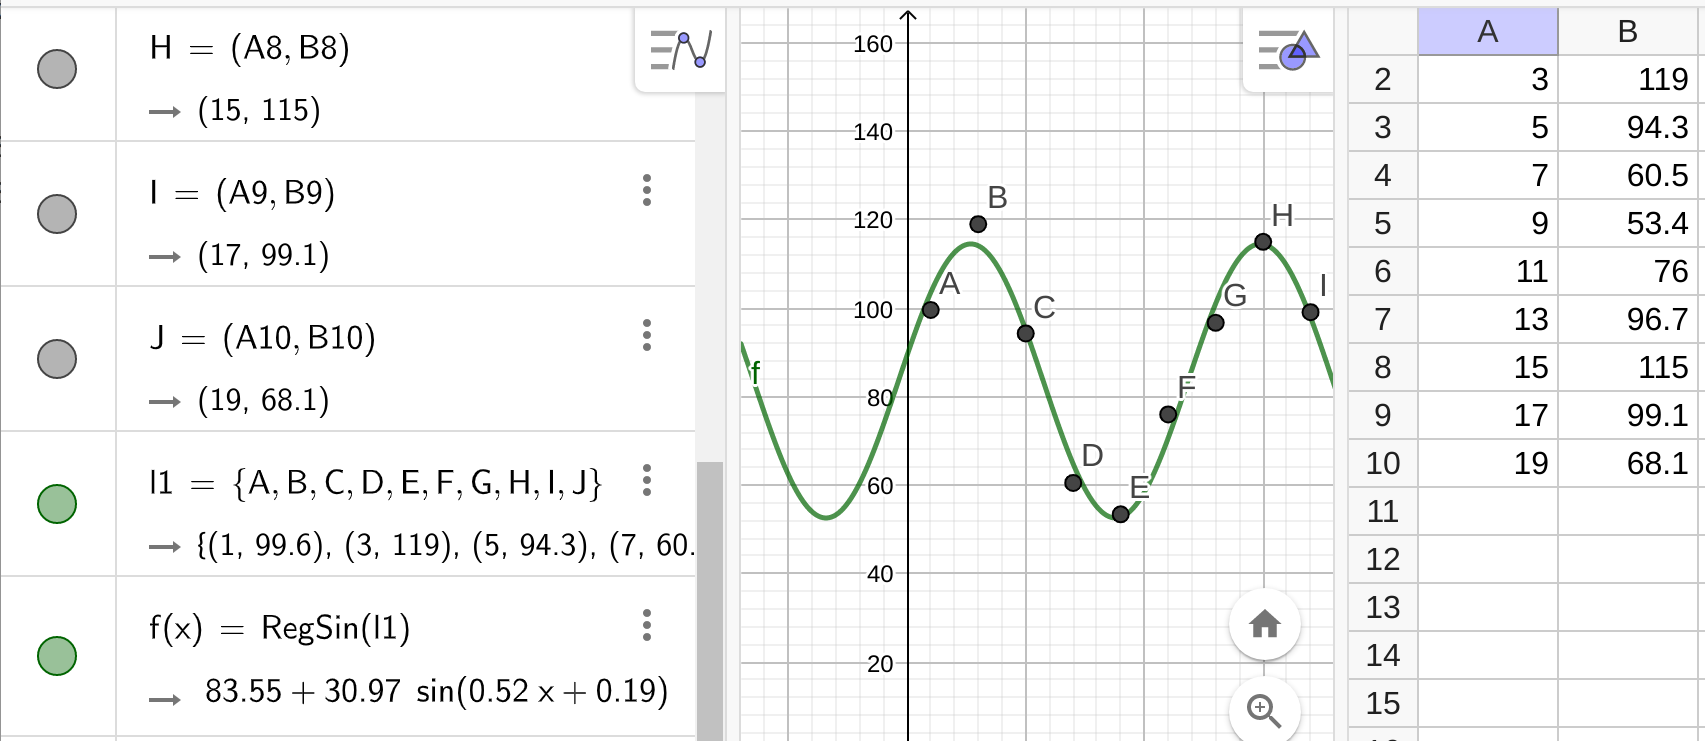
\includegraphics[scale=0.2]{opg1a}
\end{figure}

\item Ved hjelp av CAS finner vi at konsentrasjonen vil være 2.0 mmol/L etter ca. 160 sekunder.
\begin{figure}
	\centering
	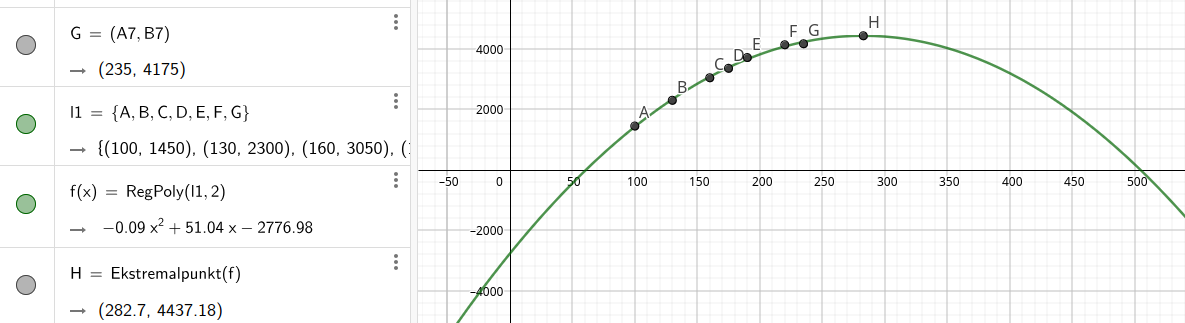
\includegraphics[scale=0.5]{opg1b}
\end{figure}
\item Ved hjelp av CAS finner vi at konsentrasjonen vil øke med mindre enn 0,001 mmol/L per sekund etter ca 321 sekunder.
\begin{figure}
	\centering
	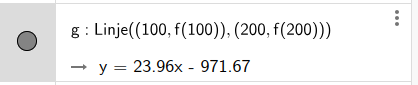
\includegraphics[scale=0.5]{opg1c}
\end{figure}
}


\newpage
\subsection*{Oppgave 2}
I CAS-celle 1 og 2 definerer vi $ g(x) $ og $ h(x) $ slik at
\[ f(x)= \left\lbrace{
	\begin{array}{rcr}
		g(x) &,&x<k \br
		h(x)   &,& x\geq k
	\end{array}
}\right. \]
\begin{figure}
	\centering
	\includegraphics[scale=0.5]{opg2ab}
\end{figure}
\abc{
\item Av celle 3 og 4 ser vi at $ \lim\limits_{x\to k} f(x) =2k $, og dermed er $ f $ kontiuerlig for alle $ k $.
\item For at $ f $ skal være deriverbar i $ x=k $, må vi at at
\[ \lim\limits_{h\to 0} \frac{g(k+h)-g(k)}{h}=\lim\limits_{h\to 0}\frac{h(k+h)-h(k)}{h} \]
Da både $ g(x) $ og $ h(x) $ er polynomer, har de en kontinuerlig deriverte funksjon for alle $ k $, og dermed er det tilstrekkelig å sjekke for hvilke verdier $ g'(k)=h'(k) $. Av celle 5 ser vi at dette bare gjelder for $ k=0 $.
\newpage
\item Da $ g(x) $ er en konkav funksjon, er den injektiv for alle $ x\in[\infty, x_m] $, hvor $ x_m $ er maksimumspunktet til $ g $. Maksimumspunktet finner vi ved å kreve at $ g'(x)=0 $ (celle 6). I tillegg må vi kreve at $ x_m<k $, som gir at $ k>2 $ (celle 7). En tilsvarende utregning med hensyn på $ h(x) $ (celle 8 og 9) gir at $ k\leq 2 $. Altså er $ f $ injektiv dersom \\$ -2\leq k<2 $.
\begin{figure}
	\centering
	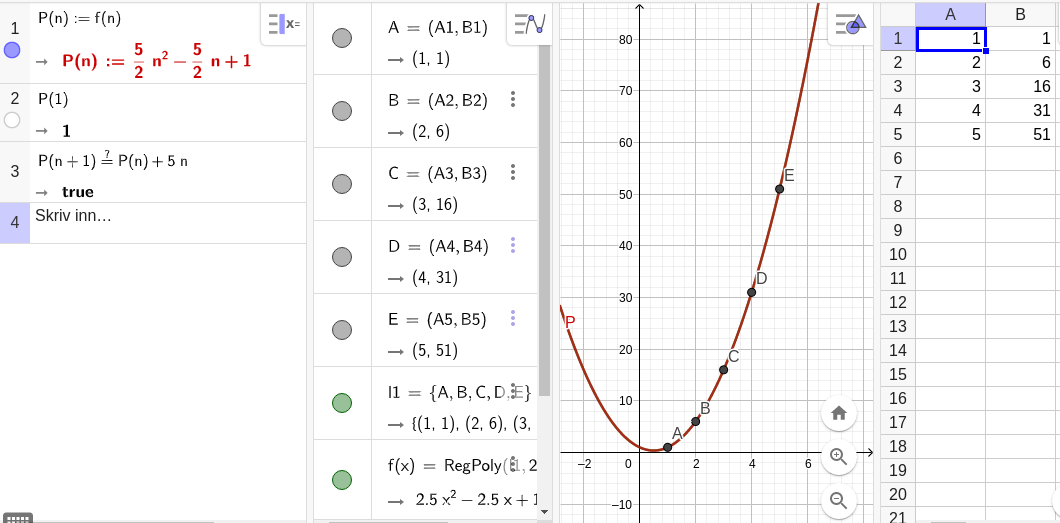
\includegraphics[scale=0.5]{opg2c}
\end{figure}
}
\newpage
\subsection*{Oppgave 3}
\abc{
\item Vi definerer tredjegradsfunksjonen $ f $ med koeffisienter $ c_1, c_2, c_3\in \mathbb{R} $ (celle 1). Ska $ f $ ha et ekstremalpunkt, må det finnes en reell løsning av ligningen $ f'(x)=0 $. Av celle 2 ser vi at hvis $ {c_2^2<3c_1c_3} $, så har ikke ligningen en rell løsning. Det er åpenbart at det finnes sett med $ c_1 $, $ c_2 $ og $ c_3 $ som oppfyller ulikheten (for eksempel $ c_1=1, c_2=0, c_3=1 $), og dermed er ikke Påstand 1 gyldig for alle sett med $ c_1 $, $ c_2 $ og $ c_3 $.
\item For at $ y=ax+b $ skal skjære $ f $, må ligningen $ f=ax+b $ ha minst én løsning. Dette er en tredjegradsligning. Alle tredjegradsligninger har minst én reell løsning, og dermed er påstand 2 riktig.
\item \textbf{Løsning 1}\\
Vi definerer $ g(x)=f'(x) $. Da $ f $ er en tredjegradsfunksjon, er $ g $ en andregradsfunksjon, og siden $ {g'(3)=0} $ er $ {(3, g(3))} $ ekstremalpunktet til $ g $. Da $ {x=1} $ og $ {x=5} $ har lik horisontalavstand til ekstremalpunktet, har vi av symmetriegenskapene til en andregradsfunksjon at $ {g(1)=g(3)} $. Altså er Påstand 3 riktig.\\[12pt]
\textbf{Løsning 2}\\
Hvis $ f $ har et vendepunkt i $ x=3 $, er $ f''(3)=0 $. Da er $ c_2=-9c_3 $ (celle 3). Vi definerer $ g(x) $ som $ f $ med koeffisienter $ c_1, c_2=-9c_3 $ og $ c_3 $ (cell 4). Da stemmer det at $ g'(x)=g'(5) $ (celle 5).
}
\begin{figure}
	\centering
	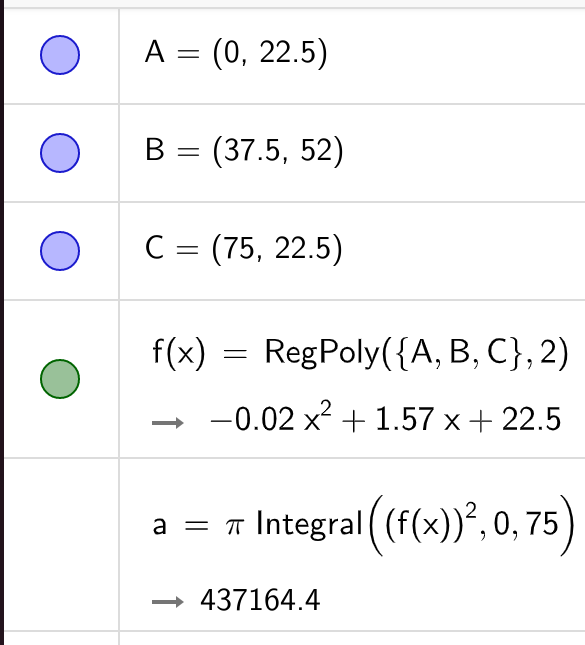
\includegraphics[scale=0.5]{opg3}
\end{figure}

\newpage
\subsection*{Oppgave 4}
Vi setter sidelengden til grunnflaten lik $ s $ og høyden lik $ h $. Da er volumet $ V $ og overflatearealet $ A $ til prismen gitt i CAS-celle 1 og 2. I celle 3 finner vi $ h $ uttrykt ved $ s $ og $ A $, og setter dette inn i $ V $ (celle 4). I celle 5 og 6 finner vi ekstremalpunktene til uttrykket fra celle 4. Da dette er et 3. gradsuttrykk med negativ koeffisient foran $ s^3 $, forventer vi at ekstremalpunktet lengst til høgre på $ x $-aksen er maksimalpunktet. Setter vi ekstremalpunktet inn i uttrykket for $ V $ (celle 7), ser vi at det største volumet oppnås ved å ha en så stor overflate som tillat.
\abc{
\item I celle 8 finner vi at det største volumet når $ {s=5} $ er $ \frac{475}{4}\enh{L}=118.75\enh{L} $.
\item I celle 9 finner vi at det maksimale volumet kassen kan få er $ 40\sqrt{10}\enh{L}\approx 126.49\enh{L} $.
\item Vi løser ligningen $ V=80 $, og får et uttrykk for $ h $ (celle 10). Deretter lager vi funksjonen $ a(s) $ (celle 11), hvor uttrykket for $ h $ er satt inn i uttrykket for $ A $ i celle 2. Da $ a $ bare har ett ekstremalpunkt (celle 12) er det ut i fra oppgaven naturlig å anta at dette er et bunnpunkt (dette kan også bekreftes av grafen til $ a $). Dermed er det minste samlede arealet platene kan ha lik $ 12\cdot20^{\frac{2}{3}}\enh{dm}^2\approx 88,42\enh{dm}^2$.
}

\begin{figure}
	\centering
	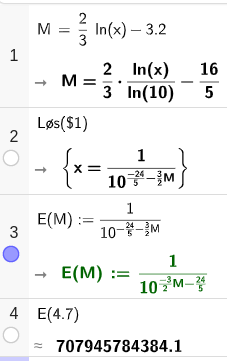
\includegraphics[scale=0.3]{opg4}
\end{figure}

\newpage
\subsection*{Oppgave 5}
\abc{
\item Vi definerer $ f(t) $ og $ g(t) $ slik at $ r(t)=[f, g] $ (celle 1, 2 og 3). $ r'(t) $ er fartsvektoren til pucken, som dermed har utgangsfart ca. lik $ 18,87\enh{m/s} $ (celle 3).
\item Vi tiden det vil ta før $ r $ antar $ x $- og $ y $-verdiene til randsonene (celle 5-8), og finner at den minste gyldige tiden er ca $ 3,05\enh{s} $. Dett er altså tiden det tok før pucken traff vantet.
\item Vi definerer posisjonsvektoren til spilleren som $ p(t) $ (celle 9), og sjekker om $ r=p $ har en løsning (celle 10). Det har den ikke, og dermed treffer ikke pucken spilleren. (Hvis vi skulle sjekket om $ p $ og $ r $ kan anta samme posisjon, måtte vi brukt to forskjellige variabler, men siden det her er snakk om samme posisjon til samme tid, kan vi bruke $ t $ for begge).
}
\begin{figure}
	\centering
	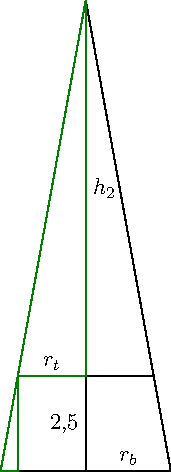
\includegraphics[scale=0.4]{opg5}
\end{figure}
\newpage
\subsection*{Oppgave 6}
\textit{Kommentar: Vi vil her presentere to løsninger. Den første løsningen fremhever viktigheten av å lese alle deloppgaver før man setter i gang med besvarelsen, og styrken av å bruke CAS så mye som mulig.
}\vsk

\textbf{Løsning 1} \\
Vi definerer $ f(x)= kx^2+lx +m $ hvor $ k, l, m\in\mathbb{R} $ (celle 1). I celle 2 har vi da et generelt uttrykk som gjelder for alle andregradsfunksjoner.
\begin{figure}
	\centering
	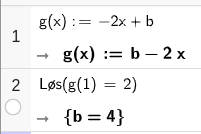
\includegraphics[scale=0.4]{opg6}
\end{figure}
\abc{
\item Av uttrykket vi har funnet er $ c=\frac{3+1}{2}=2 $.
\item Se linje 2-3 i Python-skriptet.
\item Linje 5-7 bekrefter det vi har funnet, at $ c=\frac{a+b}{2} $.
\item Da $ \frac{2+8}{2}=5 $, er Annes påstand riktig.
} \vsk

\textbf{Løsning 2}\\
Vi har at $ f'(x)=2x+3 $. Dermed er
\alg{
f'(c)&=\frac{f(b)-f(a)}{b-a} \br
2c &=\frac{f(b)-f(a)}{b-a}\br
c &= \frac{1}{2}\left(\frac{f(b)-f(a)}{b-a}-3\right)
}
\abc{
\item Vi bruker skriptet fra oppgave b) og får at $ c=2 $ (linje 8).
\item Se linje 2-6.
\item Ut i fra forsøk med tilfeldige tall ser det ut til at $ c=\frac{a+b}{2} $.
\item Gitt $ f(x)= kx^2+lx +m $ hvor $ k, l, m\in\mathbb{R} $. Ved å generalisere uttrykket vi har funnet for $ c $, får vi at
\alg{
c&= \frac{1}{2k}\left(\frac{f(b)-f(a)}{b-a}-l\right)
} 
Videre er 
\alg{
f(b)-f(a)&=kb^2+3lb+m-(ka^2+3la+m) \\
&= k(a+b)(b-a)+l(b-a)
}
Dermed er
\algv{
c&=\frac{1}{2k}k(a+b) \\
&=\frac{a+b}{2} 
}
Uttrykket gjelder altså for alle andregradsfunksjoner, og dermed er Annes påstand riktig.
}
\pythonut{meanvaluesentence_a.py}{
2.0\\
4.5\\
55.0
}
\end{document}